\documentclass[english, 11 pt, class=article, crop=false]{standalone}
\usepackage[T1]{fontenc}
%\renewcommand*\familydefault{\sfdefault} % For dyslexia-friendly text
\usepackage{lmodern} % load a font with all the characters
\usepackage{geometry}
\geometry{verbose,paperwidth=16.1 cm, paperheight=24 cm, inner=2.3cm, outer=1.8 cm, bmargin=2cm, tmargin=1.8cm}
\setlength{\parindent}{0bp}
\usepackage{import}
\usepackage[subpreambles=false]{standalone}
\usepackage{amsmath}
\usepackage{amssymb}
\usepackage{esint}
\usepackage{babel}
\usepackage{tabu}
\makeatother
\makeatletter

\usepackage{titlesec}
\usepackage{ragged2e}
\RaggedRight
\raggedbottom
\frenchspacing

% Norwegian names of figures, chapters, parts and content
\addto\captionsenglish{\renewcommand{\figurename}{Figur}}
\makeatletter
\addto\captionsenglish{\renewcommand{\chaptername}{Kapittel}}
\addto\captionsenglish{\renewcommand{\partname}{Del}}


\usepackage{graphicx}
\usepackage{float}
\usepackage{subfig}
\usepackage{placeins}
\usepackage{cancel}
\usepackage{framed}
\usepackage{wrapfig}
\usepackage[subfigure]{tocloft}
\usepackage[font=footnotesize,labelfont=sl]{caption} % Figure caption
\usepackage{bm}
\usepackage[dvipsnames, table]{xcolor}
\definecolor{shadecolor}{rgb}{0.105469, 0.613281, 1}
\colorlet{shadecolor}{Emerald!15} 
\usepackage{icomma}
\makeatother
\usepackage[many]{tcolorbox}
\usepackage{multicol}
\usepackage{stackengine}

\usepackage{esvect} %For vectors with capital letters

% For tabular
\usepackage{array}
\usepackage{multirow}
\usepackage{longtable} %breakable table

% Ligningsreferanser
\usepackage{mathtools}
\mathtoolsset{showonlyrefs}

% index
\usepackage{imakeidx}
\makeindex[title=Indeks]

%Footnote:
\usepackage[bottom, hang, flushmargin]{footmisc}
\usepackage{perpage} 
\MakePerPage{footnote}
\addtolength{\footnotesep}{2mm}
\renewcommand{\thefootnote}{\arabic{footnote}}
\renewcommand\footnoterule{\rule{\linewidth}{0.4pt}}
\renewcommand{\thempfootnote}{\arabic{mpfootnote}}

%colors
\definecolor{c1}{cmyk}{0,0.5,1,0}
\definecolor{c2}{cmyk}{1,0.25,1,0}
\definecolor{n3}{cmyk}{1,0.,1,0}
\definecolor{neg}{cmyk}{1,0.,0.,0}

% Lister med bokstavar
\usepackage[inline]{enumitem}

\newcounter{rg}
\numberwithin{rg}{chapter}
\newcommand{\reg}[2][]{\begin{tcolorbox}[boxrule=0.3 mm,arc=0mm,colback=blue!3] {\refstepcounter{rg}\phantomsection \large \textbf{\therg \;#1} \vspace{5 pt}}\newline #2  \end{tcolorbox}\vspace{-5pt}}

\newcommand\alg[1]{\begin{align} #1 \end{align}}

\newcommand\eks[2][]{\begin{tcolorbox}[boxrule=0.3 mm,arc=0mm,enhanced jigsaw,breakable,colback=green!3] {\large \textbf{Eksempel #1} \vspace{5 pt}\\} #2 \end{tcolorbox}\vspace{-5pt} }

\newcommand{\st}[1]{\begin{tcolorbox}[boxrule=0.0 mm,arc=0mm,enhanced jigsaw,breakable,colback=yellow!12]{ #1} \end{tcolorbox}}

\newcommand{\spr}[1]{\begin{tcolorbox}[boxrule=0.3 mm,arc=0mm,enhanced jigsaw,breakable,colback=yellow!7] {\large \textbf{Språkboksen} \vspace{5 pt}\\} #1 \end{tcolorbox}\vspace{-5pt} }

\newcommand{\sym}[1]{\colorbox{blue!15}{#1}}

\newcommand{\info}[2]{\begin{tcolorbox}[boxrule=0.3 mm,arc=0mm,enhanced jigsaw,breakable,colback=cyan!6] {\large \textbf{#1} \vspace{5 pt}\\} #2 \end{tcolorbox}\vspace{-5pt} }

\newcommand\algv[1]{\vspace{-11 pt}\begin{align*} #1 \end{align*}}

\newcommand{\regv}{\vspace{5pt}}
\newcommand{\mer}{\textsl{Merk}: }
\newcommand{\mers}[1]{{\footnotesize \mer #1}}
\newcommand\vsk{\vspace{11pt}}
\newcommand\vs{\vspace{-11pt}}
\newcommand\vsb{\vspace{-16pt}}
\newcommand\sv{\vsk \textbf{Svar} \vspace{4 pt}\\}
\newcommand\br{\\[5 pt]}
\newcommand{\figp}[1]{../fig/#1}
\newcommand\algvv[1]{\vs\vs\begin{align*} #1 \end{align*}}
\newcommand{\y}[1]{$ {#1} $}
\newcommand{\os}{\\[5 pt]}
\newcommand{\prbxl}[2]{
\parbox[l][][l]{#1\linewidth}{#2
	}}
\newcommand{\prbxr}[2]{\parbox[r][][l]{#1\linewidth}{
		\setlength{\abovedisplayskip}{5pt}
		\setlength{\belowdisplayskip}{5pt}	
		\setlength{\abovedisplayshortskip}{0pt}
		\setlength{\belowdisplayshortskip}{0pt} 
		\begin{shaded}
			\footnotesize	#2 \end{shaded}}}

\renewcommand{\cfttoctitlefont}{\Large\bfseries}
\setlength{\cftaftertoctitleskip}{0 pt}
\setlength{\cftbeforetoctitleskip}{0 pt}

\newcommand{\bs}{\\[3pt]}
\newcommand{\vn}{\\[6pt]}
\newcommand{\fig}[1]{\begin{figure}
		\centering
		\includegraphics[]{\figp{#1}}
\end{figure}}

\newcommand{\figc}[2]{\begin{figure}
		\centering
		\includegraphics[]{\figp{#1}}
		\caption{#2}
\end{figure}}

\newcommand{\sectionbreak}{\clearpage} % New page on each section

\newcommand{\nn}[1]{
\begin{equation}
	#1
\end{equation}
}

% Equation comments
\newcommand{\cm}[1]{\llap{\color{blue} #1}}

\newcommand\fork[2]{\begin{tcolorbox}[boxrule=0.3 mm,arc=0mm,enhanced jigsaw,breakable,colback=yellow!7] {\large \textbf{#1 (forklaring)} \vspace{5 pt}\\} #2 \end{tcolorbox}\vspace{-5pt} }
 
%colors
\newcommand{\colr}[1]{{\color{red} #1}}
\newcommand{\colb}[1]{{\color{blue} #1}}
\newcommand{\colo}[1]{{\color{orange} #1}}
\newcommand{\colc}[1]{{\color{cyan} #1}}
\definecolor{projectgreen}{cmyk}{100,0,100,0}
\newcommand{\colg}[1]{{\color{projectgreen} #1}}

% Methods
\newcommand{\metode}[2]{
	\textsl{#1} \\[-8pt]
	\rule{#2}{0.75pt}
}

%Opg
\newcommand{\abc}[1]{
	\begin{enumerate}[label=\alph*),leftmargin=18pt]
		#1
	\end{enumerate}
}
\newcommand{\abcs}[2]{
	\begin{enumerate}[label=\alph*),start=#1,leftmargin=18pt]
		#2
	\end{enumerate}
}
\newcommand{\abcn}[1]{
	\begin{enumerate}[label=\arabic*),leftmargin=18pt]
		#1
	\end{enumerate}
}
\newcommand{\abch}[1]{
	\hspace{-2pt}	\begin{enumerate*}[label=\alph*), itemjoin=\hspace{1cm}]
		#1
	\end{enumerate*}
}
\newcommand{\abchs}[2]{
	\hspace{-2pt}	\begin{enumerate*}[label=\alph*), itemjoin=\hspace{1cm}, start=#1]
		#2
	\end{enumerate*}
}

% Oppgaver
\newcommand{\opgt}{\phantomsection \addcontentsline{toc}{section}{Oppgaver} \section*{Oppgaver for kapittel \thechapter}\vs \setcounter{section}{1}}
\newcounter{opg}
\numberwithin{opg}{section}
\newcommand{\op}[1]{\vspace{15pt} \refstepcounter{opg}\large \textbf{\color{blue}\theopg} \vspace{2 pt} \label{#1} \\}
\newcommand{\ekspop}[1]{\vsk\textbf{Gruble \thechapter.#1}\vspace{2 pt} \\}
\newcommand{\nes}{\stepcounter{section}
	\setcounter{opg}{0}}
\newcommand{\opr}[1]{\vspace{3pt}\textbf{\ref{#1}}}
\newcommand{\oeks}[1]{\begin{tcolorbox}[boxrule=0.3 mm,arc=0mm,colback=white]
		\textit{Eksempel: } #1	  
\end{tcolorbox}}
\newcommand\opgeks[2][]{\begin{tcolorbox}[boxrule=0.1 mm,arc=0mm,enhanced jigsaw,breakable,colback=white] {\footnotesize \textbf{Eksempel #1} \\} \footnotesize #2 \end{tcolorbox}\vspace{-5pt} }
\newcommand{\rknut}{
Rekn ut.
}

%License
\newcommand{\lic}{\textit{Matematikken sine byggesteinar by Sindre Sogge Heggen is licensed under CC BY-NC-SA 4.0. To view a copy of this license, visit\\ 
		\net{http://creativecommons.org/licenses/by-nc-sa/4.0/}{http://creativecommons.org/licenses/by-nc-sa/4.0/}}}

%referances
\newcommand{\net}[2]{{\color{blue}\href{#1}{#2}}}
\newcommand{\hrs}[2]{\hyperref[#1]{\color{blue}\textsl{#2 \ref*{#1}}}}
\newcommand{\rref}[1]{\hrs{#1}{regel}}
\newcommand{\refkap}[1]{\hrs{#1}{kapittel}}
\newcommand{\refsec}[1]{\hrs{#1}{seksjon}}

\newcommand{\mb}{\net{https://sindrsh.github.io/FirstPrinciplesOfMath/}{MB}}


%line to seperate examples
\newcommand{\linje}{\rule{\linewidth}{1pt} }

\usepackage{datetime2}
%%\usepackage{sansmathfonts} for dyslexia-friendly math
\usepackage[]{hyperref}


\newcommand{\note}{Merk}
\newcommand{\notesm}[1]{{\footnotesize \textsl{\note:} #1}}
\newcommand{\ekstitle}{Eksempel }
\newcommand{\sprtitle}{Språkboksen}
\newcommand{\expl}{forklaring}

\newcommand{\vedlegg}[1]{\refstepcounter{vedl}\section*{Vedlegg \thevedl: #1}  \setcounter{vedleq}{0}}

\newcommand\sv{\vsk \textbf{Svar} \vspace{4 pt}\\}

%references
\newcommand{\reftab}[1]{\hrs{#1}{tabell}}
\newcommand{\rref}[1]{\hrs{#1}{regel}}
\newcommand{\dref}[1]{\hrs{#1}{definisjon}}
\newcommand{\refkap}[1]{\hrs{#1}{kapittel}}
\newcommand{\refsec}[1]{\hrs{#1}{seksjon}}
\newcommand{\refdsec}[1]{\hrs{#1}{delseksjon}}
\newcommand{\refved}[1]{\hrs{#1}{vedlegg}}
\newcommand{\eksref}[1]{\textsl{#1}}
\newcommand\fref[2][]{\hyperref[#2]{\textsl{figur \ref*{#2}#1}}}
\newcommand{\refop}[1]{{\color{blue}Oppgave \ref{#1}}}
\newcommand{\refops}[1]{{\color{blue}oppgave \ref{#1}}}
\newcommand{\refgrubs}[1]{{\color{blue}gruble \ref{#1}}}

\newcommand{\openmathser}{\openmath\,-\,serien}

% Exercises
\newcommand{\opgt}{\newpage \phantomsection \addcontentsline{toc}{section}{Oppgaver} \section*{Oppgaver for kapittel \thechapter}\vs \setcounter{section}{1}}


% Sequences and series
\newcommand{\sumarrek}{Summen av en aritmetisk rekke}
\newcommand{\sumgerek}{Summen av en geometrisk rekke}
\newcommand{\regnregsum}{Regneregler for summetegnet}

% Trigonometry
\newcommand{\sincoskomb}{Sinus og cosinus kombinert}
\newcommand{\cosfunk}{Cosinusfunksjonen}
\newcommand{\trid}{Trigonometriske identiteter}
\newcommand{\deravtri}{Den deriverte av de trigonometriske funksjonene}
% Solutions manual
\newcommand{\selos}{Se løsningsforslag.}
\newcommand{\se}[1]{Se eksempel på side \pageref{#1}}

%Vectors
\newcommand{\parvek}{Parallelle vektorer}
\newcommand{\vekpro}{Vektorproduktet}
\newcommand{\vekproarvol}{Vektorproduktet som areal og volum}


% 3D geometries
\newcommand{\linrom}{Linje i rommet}
\newcommand{\avstplnpkt}{Avstand mellom punkt og plan}


% Integral
\newcommand{\bestminten}{Bestemt integral I}
\newcommand{\anfundteo}{Analysens fundamentalteorem}
\newcommand{\intuf}{Integralet av utvalge funksjoner}
\newcommand{\bytvar}{Bytte av variabel}
\newcommand{\intvol}{Integral som volum}
\newcommand{\andordlindif}{Andre ordens lineære differensialligninger}


\begin{document}


\section{Introduksjon til differensialligninger\label{difgen}}
Vi er fra tidligere vant med ligninger hvor vi søker ett eller flere ukjente tall som oppfyller krav formulert ved de fire elementære regneartene multiplikasjon, divisjon, addisjon og subtraksjon. Når vi nå skal gå over til \textit{differensialligninger}\index{differensialligning}, skal vi i tillegg stille krav ved hjelp av derivasjon, og vi skal anvende integrasjon\footnote{Vi tar opp tråden fra forrige kapittel, hvor størrelser betegnet med store bokstaver tas for å være konstanter (så lenge ikke annet er nevnt).}\footnote{I tilfeller hvor den antideriverte er et $\ln $-uttrykk, dropper vi her å skrive tallverdier. Å ta med tallverdier gjør utregninger vanskeligere, men har ingen betydning for det endelige svaret.} for å løse ligningene. \vsk

Fordi derivasjon setter premissene for en differensialligning, er det viktig å innse at løsningen vi søker er en funksjon. Det er vanlig å kalle denne funksjonen for $ y$. I tilfellene vi skal se på er $ y $ avhengig av én variabel, oftest beskrevet av bokstaven $ x $ eller $ t $.

\subsection{Første ordens ligninger}
Den enkleste differensialligningen er følgende:
\begin{equation}
y'=0  \label{enkleste}
\end{equation}
Fordi den førstederiverte er den høyeste graden av derivasjon i ligningen, kaller vi den for en \textit{første ordens}\index{differensialligning!første ordens} differensialligning. Hvis vi lar $ x $ være den frie variablen, kan vi integrere begge sider mhp. $ x $:
\[ \int y' \,dx = \int 0 \,dx \]
Siden $ y $ er en antiderivert til $ y' $, kan vi skrive
\begin{equation}
y = C \label{enklestel}
\end{equation}
Også for differensialligninger kan vi selvsagt sjekke at løsningen vår er riktig, og det bør ikke ta deg lang tid å sjekke at (\ref{enklestel}) oppfyller kravet fra (\ref{enkleste}).\vsk

Det vi fant over kan kanskje virke trivielt, men faktisk har vi allerede avdekket en viktig egenskap: Fordi $ C $ er en vilkårlig konstant, må (\ref{enkleste}) ha uendelig mange løsninger! Dette gjelder for alle differensialligningene vi skal se på i dette kapittelet. Når vi ikke har bestemt konstanten(e) enda, har vi har funnet den \textit{generelle} løsningen.\vsk

Skal vi bestemme konstantene trenger vi mer informasjon, som oftest i form av at vi vet hva $ y$ eller dens deriverte er for noen verdier av $ x $. Slik informasjon kalles gjerne \textit{randbetingelser}\index{randbetingelse} eller \textit{initialkrav}\index{initialkrav}\footnote{Randbetingelse brukes gjerne når den frie variabelen har en romlig dimensjon, mens initialbetingelse brukes oftest hvis den har tidsdimensjon.}. For eksempel: Om vi angående vår $ y $ fra (\ref{enklestel}) vet at $  {y(0)=1 }$, finner vi fort at $ {C=1} $.

\subsection{Andre ordens ligninger}
Da $ {y'=0 }$ var så grei å håndtere, er det fristende å også prøve seg på ligningen
\[ y''=0 \]
Fordi den andrederiverte her er den høyeste orden av derivasjon, kalles dette en \textit{andre ordens}\index{differensialligning!andre ordens} differensialligning. Om vi ved to tilfeller integrerer begge sider mhp. $ x $, får vi at
\begin{align}
	\int y''\, dx &= \int 0 \, dx \nonumber\\
	y' &= C \nonumber\\
	\int y'\, dx &= \int C \, dx \nonumber\\
	y &= Cx + D
\end{align}
Og atter en gang har det vi kan tillate oss å kalle for en enkel ligning gitt en pekepinne mot et viktig faktum; for den typen andre ordens differensialligninger som omtales i \refsec{sode} forventer vi nemlig også to konstanter som ikke kan slås sammen til én.

\section[Første ordens lineære differensialligninger]{Første ordens lineære differensial- \\ ligninger\label{fode}}
La oss nå undres om det finnes en funksjon $ y(x) $ som er slik at den deriverte av funksjonen, addert to ganger funksjonen selv, tilsvarer tallet 6:
\begin{equation}
 y'+2y=6 \label{diff1}
\end{equation}
Ligningen over kalles en \textit{første ordens lineær}\index{differensialligning!første ordens!lineær} differensialligning. Begrepet lineær kommer av at hverken $ y $ eller funksjones deriverte er av høyere potens enn én. Hadde vi for eksempel hatt $ (y')^4 $ med i ligningen, ville den vært en \textit{første ordens ikke-lineær} differensialligning.\vsk

De fleste ikke-lineære ligninger er veldig vanskelige å løse eksakt, mens lineære ligninger som (\ref{diff1}) greier vi fint å håndtere. Er du dreven i derivering ser du kanskje at funskjonen ${y= e^{-2x}+3} $ vil oppfylle ligningen \vs
\alg{
\overbrace{(e^{-2x}+3)'}^{y'}+2\overbrace{\left(e^{-2x}+3\right)}^{2y} =4 \\
-2e^{-2x}-2e^{-2x}+6 = 6 \\
6=6
}
Å tippe eller se svar er absolutt lov å gjøre, men ikke alltid så enkelt. Dessuten nevnte vi jo i forrige seksjon at det forventes uendelig mange løsninger, altså en generell løsning. Denne skal vi finne ved å gå fram på en mer systematisk måte.\vsk

Vi starter med å gange begge sider av ligningen med $ e^{2x} $:
\begin{equation}
y'e^{2x}+2ye^{2x}=6e^{2x} \label{diff1a}
\end{equation}
Av produktregelen ved derivasjon (se (\ref{prreg})) merker vi oss at
\[ \left(ye^{2x}\right)'=y'e^{2x}+2ye^{2x} \]
Uttrykket på høyresiden over er identisk med venstresiden i (\ref{diff1a}), dermed er
\[ \left(ye^{2x}\right)'= 6e^{2x}\]
Et uttrykk for $ y $ kan vi nå finne ved å integrere mhp. $ x $:
\alg{
\int \left(ye^{2x}\right)' \, dx&= \int 6e^{2x} \, dx \\
ye^{2x} &= 3e^{2x} + C \\
y &= 3 + Ce^{-2x}
}
Dette er den generelle løsningen av ligningen. For å tydeliggjøre at\\ $ y= {Ce^{-2x} +3} $ er riktig løsning uavhengig av verdien til \textit{C}, kan vi sette dette uttrykket for \textit{y} inn i (\ref{diff1})\footnote{Som du trolig er vant med fra tidligere, kalles dette å sette prøve på svaret.}:
\alg{
(Ce^{-2x}+3)' + 2(Ce^{-2x}+3) &=6 \\
 - 2Ce^{-2x} +2Ce^{-2x}+6 &=6\\
2C(e^{-2x}-e^{-2x})+6&=6 \\
6&=6
}
Ligningen er dermed oppfylt.\regv
\newpage
\reg[Første ordens lineære differensialligninger]{
	Ligninger på formen 
	\[ y'+f(x)y=g(x)  \]
	kan løses ved å multiplisere ligningen med \textit{den integrerende faktoren} $ e^{F(x)} $, hvor $ F $ er den antideriverte av $ f $ (uten konstantledd). Man kan da omskrive ligningen til
	\[ \left(ye^{F(x)}\right)'=g(x)e^{F(x)} \]
	som kan løses ved integrasjon.
}
\eks[1]{
	Gitt differensialligningen
	\[ y'-2xy=6x \]
	\textbf{a)} Finn den generelle løsningen av ligningen. \os
	\textbf{b)} Finn løsningen som oppfyller randbetingelsen $ y(0)=0 $.
	
	\sv
	\textbf{a)} Uttrykket foran $ y $ er lik $ -2x $, den antideriverte blir derfor $ -x^2 $ og den integrerende faktoren blir da $ e^{-x^2} $
	\alg{
		(y' -2xy)e^{-x^2}&= 6x e^{-x^2} \\
		\int (y' -2xy)e^{-x^2} \,dx &= \int 6x e^{-x^2}\, dx \\
		\int \left(ye^{-x^2}\right)' \,dx &= \int 6x e^{-x^2}\, dx \\
		ye^{-x^2} &= -3 e^{-x^2} +C \\
		y &= -3  +Ce^{x^2}
	}
	\textsl{Merk:} Her er bytte av variabel brukt for å løse integralet på høyresiden i ligningen over. \vsk
	
	\textbf{b)} \algv{y(0)&=-3+Ce^{0^2} \\
		0 &= -3+C \\
		3 &= C
	}
	Løsningen som oppfyller randbetingelsen er altså
	\[ y=3(e^{x^2}-1) \]\vs
}
\eks[2]{
Løs ligningen
\[ y'-y+x=0 \] \vs
\sv
Uttrykket foran $ y $ er $ -1 $, den integrerende faktoren blir derfor $ e^{-x} $\,:
\algv{
y'-y &= -x \\
(y'-y)e^{-x}&= -xe^{-x} \\
\left(ye^{-x}\right)' &= -xe^{-x} \\
\int \left(ye^{-x}\right)' \,dx&= \int -xe^{-x}\,dx \\
ye^{-x}&= xe^{-x}-\int e^{-x}\,dx \\
ye^{-x} &=xe^{-x}+ e^{-x}+ C \\
y &=x+ 1+ Ce^{x} 
}
\textsl{Merk}: Delvis integrasjon ble brukt for å finne integralet på høyre side i ligningen over.
}
\section{Separable differensialligninger}\index{differensialligning!separabel}
La oss nå se på differensialligningen \[ y'+3y^4= 0 \]
Her kan vi ikke bruke løsningsmetoden fra forrige seksjon, isteden omskriver vi ligningen til
\[ \frac{y'}{y^4}=-3 \]
En ligning som kan omskrives slik at vi får $ y' $ av første orden og enhver funksjon av $ y $ samlet på èn side, kalles en \textit{separabel differensialligning}.\vsk

Vi fortsetter ved å integrere mhp. $ y $:
\[\int \frac{y'}{y^4} \,dx=\int -3 \, dx\]
Integralet på venstresiden kan vi skrive om til (se (\ref{bytvar}))
\[ \int \frac{y'}{y^4} \,dx= \int \frac{1}{y^4}\,dy  \]
Vi får derfor at
\alg{
\int \frac{1}{y^4} \,dy&=\int -3 \, dx \br
-\frac{1}{3}y^{-3} &= -3 x +C\\
y^{-3}&= 9 x + C \\
\left(y^{-3}\right)^{-\frac{1}{3}} &= (9x+ C)^{-\frac{1}{3}}\\
y &= (9x+ C)^{-\frac{1}{3}}
	}
\reg[Separable differensialligninger]{Enhver ligning som kan skrives på formen 
	\begin{equation}\label{sep}
		{g(y)y' = f(x)} 
	\end{equation} er en separabel differensialligning. Ligningen kan løses ved å integrere mhp. $ x $ på begge sider:
	\alg{
		\int g(y)y' \, dx &= \int f(x) \, dx \\
		\int g(y) \, dy &= \int f(x) \, dx	
	}
	og deretter løse ligningen for $ y $.	
}
\newpage
\eks{
	Finn den generelle løsningen for differensialligningen
	\[ y' + 8xy=0 \]
	
	\sv
	Vi starter med å separere ligningen:
	\alg{
		y' + 8xy &=0 \\
		\frac{y'}{y}&=-8x
	}
	Vi integrerer så på begge sider mhp $ x $ og løser deretter for $ y $:
	\alg{\int \frac{y'}{y} \,dx&=\int-8x\, dx \\
		\int \frac{1}{y}\, dy &= -4x^2 +C\\
		\ln y &= -4x^2 +C \\
		e^{\ln y} &= e^{-4x^2 + C} \\
		y &= e^{-4x^2 + C} \\
		&= De^{-4x^2}
	}
	\textsl{Merk}: $ {D=e^C} $.
}
\section{Retningsdiagram}
Så langt har vi funnet det som kalles \textit{analytiske} løsninger av forskjellige differensialligninger, dette innebar at løsningene hadde eksakte uttrykk. Men for de aller fleste differensialligninger har vi faktisk ikke teknikker som sikrer oss analytiske løsninger, og da må vi nøye oss med tilnærminger.\vsk

Vi skal her se på en teknikk som innebærer at vi prøver å utnytte ''oppførselen'' til løsningene. Vi starter med å late som at vi ikke greier å løse ligningen
\begin{equation}
y'+x^2 y = 0 \label{retn0}
\end{equation}
Men istedenfor å gi opp, isolerer vi $ y' $:
\[ y'= -x^2 y \]
Nå har vi et uttrykk for $ y' $ for et hvilket som helst punkt $ (x, y) $. I tillegg vet vi at $ y'(x,y) $ er stigningstallet til tangenten til $ y $ i punktet $ (x, y) $. Så hvis vi nå tegner inn tangentene til mange forskjellige kombinasjoner av $ x $ og $ y $, vil vi forhåpentligvis se en trend. Figuren vi da får kalles et \textit{retningsdiagram}\index{retningsdiagram}.
\begin{figure}
		\centering
	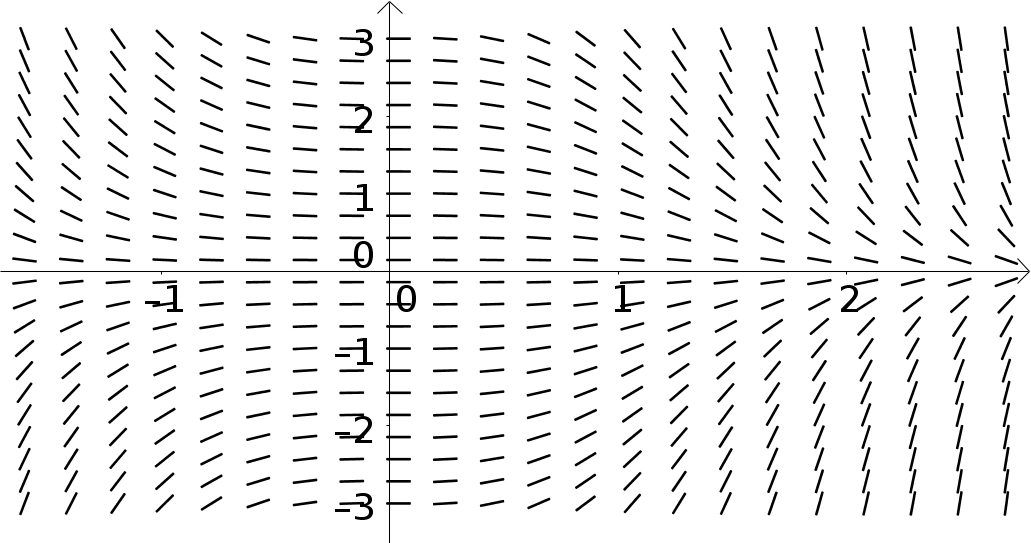
\includegraphics[scale=1]{retn}
	\caption{Tangenten til $ y $ i punktet $ (x, y) $ for kombinasjonene av 31 forskjellige verdier av $ x $ og $ y $. \label{retn}}
\end{figure}
Vi har sett at differensialligninger har uendelig mange løsninger. Ut ifra \fref{retn} ser det ut til at tallverdien til enhver $ y $
\begin{itemize}
	\item avtar forholdsvis kraftig fram til $ x $ nærmer seg ca. $ -1 $ fra negativ side av tallinja.
	\item forblir tilnærmet konstant i området rundt $ x=0 $.
	\item nærmer seg stadig mot 0 for økende verdier av $ x $.
\end{itemize}
Men nå vet vi jo at den generelle løsningen til (\ref{retn0}) er $ y=Ce^{-\frac{1}{3}x^3} $. For å bekrefte vår beskrivelse av oppførselen, kan vi derfor tegne inn grafen til løsningene for $ {C=2} $ og $ {C=-1} $:
\newpage
\begin{figure}
		\centering
	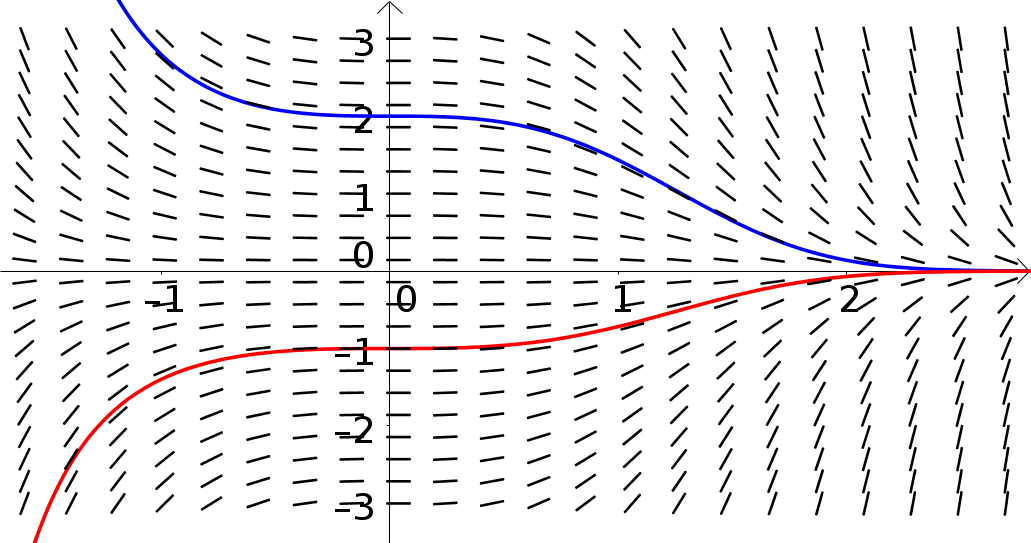
\includegraphics[scale=1]{retn2}
	\caption{Løsningene (integralkurvene) $ {y=2e^{-\frac{1}{3}x^3}} $ (blå) og $ {y=-e^{-\frac{1}{3}x^3}} $ (rød) tegnet inn i retningsdiagrammet.}
\end{figure}
Kurvene til bestemte løsninger av differensialligninger kalles \textit{integralkurver}. \index{integralkurver}
\eks{
Gitt differensialligningen 
\[ x^2y'+3y = 4x \]	
\textbf{a)} Finn et uttrykk for $ y' $. \os
\textbf{b)} Finn stigningstallet til $ y $ i punktene $ (1, 1) $ og $ (-1, 2) $.

\sv
\textbf{a)}\algv{x^2y'&=4x-3y \\
	y' &= \frac{4x-3y}{x^2}
	}
\textbf{b)} Stigningstallet er verdien til $ y' $ i hvert av punktene:\alg{
	y'(1, 1) &= \frac{4\cdot1-3\cdot1}{1^2} \\
	&= 1 \\[5pt]
	y'(-1, 2) &= \frac{4\cdot(-1)-3\cdot2}{(-1)^2} \\
	&= -10 	 
	}
\vs
}
\newpage
\section[Andre ordens lineære differensialligninger]{Andre ordens lineære differensial- \\ ligninger\label{sode}}
Vi ønsker nå å løse ligningen
\begin{equation}
ay''+by'+cy=0 \label{sodeeq}
\end{equation}
hvor $ a $, $ b $ og $ c $ er konstanter. Dette er en \textit{andre ordens lineær}\index{differensialligning!andre ordens!lineær} differensialligning. Fordi $ y $ og funksjonens deriverte inngår i alle ledd forskjellige fra 0, betegnes den i tillegg som \textit{homogen}\index{homogen}.\vsk

For de lineære ligningene vi så på i \refsec{fode} var eksponentialfuksjonen alltid en del av løsningen. Dette, i tillegg til funksjonens særegne egenskap ved derivasjon, gjør at det er naturlig å sjekke om den er innblandet også her. Vi setter derfor $ {y=e^{rx} }$, for en konstant $ r $, inn i (\ref{sodeeq}). Da får vi at
\begin{align}
	a\left(e^{rx}\right)''+b\left(e^{rx}\right)'+ e^{rx} &= 0\nonumber \\
	ar^2e^{rx}+ bre^{rx} + ce^{rx}&= 0\nonumber\\
	\left(ar^2 + br + c\right)e^{rx} &= 0 \tag{$ e^{rx}\neq 0 $}\nonumber \\
	ar^2 + br + c &= 0 \label{sodkar}
\end{align}
Ligning (\ref{sodeeq}) er derfor oppfylt hvis vi kan finne en $ r $ som oppfyller andregradsligningen over. \eqref{sodkar} kalles den \textit{karakteristiske ligningen}\index{karakteristisk ligning} til \eqref{sodeeq} og kan løses ved \textit{abc-formelen}:
\[ r = \frac{-b\pm\sqrt{b^2-4ac}}{2a} \]
I tidligere skolematematikk har vi sagt at \eqref{sodkar} ikke har en \textit{reell} løsning\footnote{Mange tekster opererer også med at ligningen ikke har noen løsning.}\label{rkmpstart} når  ${ b^2-4ac<0 }$, og stoppet der. Men det viser seg at vi går glipp av mange løsninger av (\ref{sodeeq}) om vi ikke også tar med de \textit{komplekse} løsningene\index{kompleks!løsning} av \eqref{sodkar}.\vsk

I \textit{kompleks analyse} innfører man bokstaven 'i' for å betegne kvadratroten av $( -1) $:
\[ \mathrm{i}=\sqrt{-1} \]
Et tall som $ 3+5\sqrt{-1} $ kalles et \textit{komplekst tall}\index{kompleks!tall}, og skrives gjerne som \\$ 3+5\mathrm{i} $.\vsk

La oss som et eksempel se hvilken konsekvens kompleks analyse har for ligningen
\[ r^2 +9 = 0  \]
Fra ethvert tall kan vi alltid faktorisere ut $ (-1) $, med introduksjonen av 'i' får vi derfor at
\alg{
	r^2 &= -9 \\
	r^2 &= 9(-1) \\
	r &= \pm \sqrt{9(-1)}\\
	&= \pm \sqrt{9}\sqrt{-1}\\
	&= \pm 3\mathrm{i}
	}
Den \textit{komplekse løsningen}\index{kompleks!løsning} er altså $ r=\pm 3\mathrm{i} $.\vsk

Med kjennskapen til komplekse tall er vi klare til å se på alle løsninger av (\ref{sodeeq}):
\reg[\andordlindif \label{andordlindif}]{
	En differensialligning på formen
	\begin{equation}
		ay'' +by'+cy=0 \label{2ord}
	\end{equation}
	har karakteristisk ligning
	\begin{equation}
		ar^2 + br + c=0 \label{rlig}
	\end{equation} 
	\textbf{To løsninger:}\\
	Hvis (\ref{rlig}) har to løsninger $ {r=r_1} $ og ${r=r_2} $, har (\ref{2ord}) løsningen
	\begin{equation}
		y = Ce^{r_1 x} + De^{r_2 x} \label{tore}
	\end{equation}
	
	\textbf{Én løsning:}\\
	Hvis (\ref{rlig}) bare har èn løsning ${r= r_1} $, har (\ref{2ord}) løsningen
	\begin{equation}
		y = Ce^{r_1x}+xDe^{r_1x} \label{enre}
	\end{equation}
	
	\textbf{Kompleks løsning:}\\
	Hvis \eqref{rlig}	har kompleks løsning $ {r = p \pm q\mathrm{i}} $, hvor $ {\mathrm{i}=\sqrt{-1}} $, kan den reelle løsningen til \eqref{2ord} skrives som
	\begin{equation}
		y=e^{px}(C\cos (qx) + D \sin (qx)) \label{kompleks}
	\end{equation}\vs
}
\eks[1]{
	Gitt differensialligningen
	\[ y''+3y'-10y=0  \]
	\textbf{a)} Finn den generelle løsningen \os
	\textbf{b)} Finn løsningen som oppyller randbetingelsene $ {y(0)=3 }$ og $ {y'(0)=-1 }$. 
	
	\sv
	\textbf{a)} Den karakteristiske ligningen blir
	\[ r^2+3r-10=0 \]
	Siden $ (-2)5=-10 $ og $ (-2)+5=3 $, kan vi skrive
	\[ r^2+3r-10 = (r-2)(r+5) \]
	Den karakteristiske ligningen har derfor løsningene $ {r=2} $ og $ {r=-5} $. Den generelle løsningen blir da
	\[ y = Ce^{2x}+De^{-5x} \]
	\textbf{b)} Fra den første randbetingelsen har vi at
	\alg{
		y(0) &= 3 \\
		Ce^{2\cdot 0}+ De^{-5\cdot 0} &= 3 \\
		C + D &= 3 \tag{I}\label{x1}
	}
	For å bruke den andre randbetingelsen må vi finne $ y' $:
	\[ y' = 2Ce^{2x}-5De^{-5x} \]
	Videre er \vs
	\alg{
		y'(0) &= -1 \\
		2Ce^{2\cdot 0}-5De^{-5\cdot 0} &= -1\\
		2C-5D &= -1 \tag{II}\label{x2}
	}
	Når vi løser ligningssettet dannet av (\ref{x1}) og (\ref{x2}), finner vi at $ {C=2} $ og $ {D=1} $. Løsningen vi søker er altså
	\[ y = 2e^{2x}+e^{-5x} \]\vs
}
\eks[2]{
	Finn den generelle løsningen av ligningen
	\[ 2y''+8y'+8y=0 \] \vs
	\sv
	Den karakteristiske ligningen blir
	\[ 2r^2 + 8r + 8 = 0 \]
	Videre er
	\alg{
		r^2 + 4r + 4&= 0 \\
		(r+2)^2 &= 0
	}
	Altså har vi bare løsningen $ {r=-2} $. Den generelle løsningen av differensialligningen blir derfor
	\[ y = (C+Dx)e^{-2x} \]
}
\eks[3]{
	Finn den generelle løsningen av ligningen
	\[ y''-4y' + 13y = 0 \] \vs
	\sv
	Den karakteristiske ligningen blir
	\[ r^2-4r+13 = 0 \]
	Denne ligningen har ingen åpenbart enkel løsning, så her må vi ta i bruk \textit{abc}-formelen:
	\alg{
		r &=\frac{ -(-4) \pm \sqrt{(-4)^2-4\cdot1\cdot13}}{2\cdot1} \\
		r &=\frac{ 4 \pm \sqrt{-36}}{2} \\
		r &=\frac{ 4 \pm \sqrt{36}\sqrt{-1}}{2} \\
		r &=\frac{ 4 \pm 6\mathrm{i}}{2} \\
		r &= 2 \pm 3\mathrm{i}
	}
	Her får vi komplekse verdier for $ r $, og dermed følgende generelle løsning:
	\[ y = e^{2x}(C\cos 3x+D\sin 3x) \]\vs
}


\tsec{Forklaringer}
\fork{\ref{andordlindif} \andordlindif}{
I \refsec{sode} har vi sett at ligningen
\begin{equation}
	ay''+by'+cy = 0 \label{sodeforkl}
\end{equation}
har ${y= e^{rx}} $ som løsning hvis $ r $ oppfyller den karakteristiske ligningen
\begin{equation}
	ar^2 + br + c = 0 \label{kar}
\end{equation}
I tillegg ble det nevnt i seksjon \ref{difgen} at vi for disse typen ligninger forventer en generell løsning som består av to konstanter vi ikke kan slå sammen til én. Mer nøyaktig forventer vi at løsningen er en \textit{lineærkombinasjon}\index{lineærkombinasjon} av to \textit{lineært uavhengige}\index{lineært uavhengig} funksjoner, men hverken disse to begrepene eller et bevis for dette skal vi bruke tid på her. Isteden skal vi se noe overfladisk på hvorfor løsningene blir så forskjellige for de tre tilfellene av den karakteristiske ligningen. \vsk

Vi starter med å vise at hvis $ {y=y_1} $ og $ {y=y_2} $ er to løsninger av (\ref{sodeforkl}), så er $ {y=y_1 + y_2 }$ også en løsning:
\alg{
	a(y_1+y_2)''+b(y_1+y_2)'+c(y_1+y_2) &= 0	 \\
	ay_1''+ay_2''+ by_1'+by_2' + cy_1+cy_2 &= 0 \\
	\underbrace{ay_1''+ by_1' + cy_1}_{0}+\underbrace{ay_2''+by_2'+cy_2}_{0} &= 0
}
Med samme framgangsmåte kan vi også vise (prøv selv!) at hvis $ {y=y_1} $ er en løsningen, må $ y=Cy_1 $ også være det. \vsk

Av det som er drøftet over, er målet nå å finne to funksjoner $ y_1 $ og $ y_2 $ som begge oppfyller (\ref{sodeforkl}), og som er slik at $ {y_1\neq Dy_2} $. Da vil nemlig $ {y=Cy_1+Dy_2} $ være den komplette løsningen av differensialligningen.\vsk

\textbf{To reelle røtter}\bs
Når (\ref{kar}) har to distinkte og reelle røtter $ {r=r_1} $ og $ {r=r_2} $, betyr dette at både $ {y_1=e^{r_1x}} $ og $ {y_2=e^{r_2x} }$ er løsninger av (\ref{sodeforkl}). Da må også både $ {y_1=Ce^{r_1x}} $ og $ {y_2=De^{r_2x}}$ være løsninger av differensialligningen. Og fordi $ r_1\neq r_2 $, må vi ha at $ Ce^{r_1 x}\neq De^{r_2 x} $. Den generelle løsningen vi søker er dermed
\[ y=Ce^{r_1}+De^{r_2}   \]

\textbf{Én reell rot}\bs
Hvis (\ref{kar}) har én rot $ {r=r_1} $, er $ {y=e^{r_1x}} $ en løsning av \eqref{sodeforkl}. Men om vi som i tilfellet av to reelle røtter legger sammen løsningene ${y_1 =Ce^{r_1x}} $ og ${y_2= De^{r_1x}} $, ender vi opp med løsningen $ {y=(C+D)e^{r_1 x} }$. Dette motstrider det løselig definerte kravet vårt om to konstanter som ikke kan slås sammen til én for å ha en komplett løsning.\vsk

Dette motiverer oss til å søke en løsning på formen $ {y=u(x)e^{r_1x} }$, hvor $ u $ er en ukjent funksjon av $ x $.
Når $ {r=r_1} $ er den eneste løsningen av den karakteristiske ligningen, må denne være på formen
\[ (r-r_1)^2=r^2-2r_1r+r_1^2=0  \]
Dette betyr at differensialligningen kan skrives som
\[ y''-2r_1 y'+r_1^2y=0 \]
Setter vi $ y=u(x)e^{r_1x} $ inn i ligningen over, får vi at
\alg{
	\left(ue^{r_1x}\right)''-2r_1 \left(ue^{r_1x}\right)'+r_1^2ue^{r_1x}&=0 \br
	\left((u'+r_1u)e^{r_1x}\right)'-2r_1(u'+r_1u)e^{r_1x} + r_1^2ue^{r_1x} &=0 \br
	\left((u''+r_1u')+r_1(u'+r_1u)-2r_1(u'+r_1u) + r_1^2u\right)e^{r_1x}&=0 \tag{$ e^{r_1x}\neq0 $}\br
	u''+r_1u'+r_1(u'+r_1u)-2r_1(u'+r_1u) + r_1^2u &=0 \br
	u'' &= 0
}
Ved integrasjon to ganger finner vi at $ u=C+Dx $, og dermed at 
\[ y = (C+Dx)e^{r_1x} \]
\textbf{To komplekse røtter}\bs
Det kan kanskje virke litt rart at alle løsninger av (\ref{sodeforkl}) hittil har bestått av eksponentialfunksjonen\index{eksponentialfunksjon}, mens vi i tilfellet av to komplekse røtter ender opp med en kombinasjon av sinus og cosinus. Men for to komplekse røtter $ {r= p+\mathrm{i}q}$ og $ {r= p-\mathrm{i}q}$ får vi faktisk en generell løsning på akkurat samme formen som for tilfellet av to reelle røtter:
\alg{y &= \hat{C}e^{(p+\mathrm{i}q)x}+\hat{D}e^{(p-\mathrm{i}q)x}\\&=e^{px}(\hat{C}e^{\mathrm{i}qx}+\hat{D}e^{-\mathrm{i}qx}) }
Til forskjell tillates her komplekse verdier\index{kompleks!verdi} også for de vilkårlige konstantene, noe som er indikert ved symbolet '$ \;\hat{}\; $'. Men skal differensialligningen brukes til å modellere fysiske systemer fra virkeligheten, må vi sørge for at løsningen er reell. For å utrette dette anvender vi \textit{Eulers formel}:
\[ \phantom{aaaaaa}e^{\mathrm{i}qx}=\cos(qx)+\mathrm{i}\sin(qx) \tag{\text{Eulers formel}}\]
Av denne kan vi skrive (husk at $ {\cos(-x)=\cos x} $ og at $ {\sin(-x)=-\sin x} $)
\small \alg{
	\hat{C}e^{\mathrm{i}qx}+\hat{D}e^{-\mathrm{i}qx} &= \hat{C}(\cos(qx)+\mathrm{i}\sin(qx))+ \hat{D}(\cos(-qx)+\mathrm{i}\sin(-qx))	\\
	&= (\hat{C}+\hat{D})\cos(qx)+\mathrm{i}(\hat{C}-\hat{D})\sin(qx)
}
\normalsize
Ved riktig valg\footnote{Vi lar $ \hat{C}=a+\mathrm{i}b $ og $ \hat{D}=a-\mathrm{i}b $, hvor $ a $ og $ b $ er to reelle konstanter.} av $ \hat{C} $ og $ \hat{D} $ kan vi lage oss de reelle tallene $ {C=\hat{C}+\hat{D}}  $ og $ D=\hat{C}-\hat{D} $, og med det få den reelle løsningen
\[ y =  e^{px}(Ccos (qx) + D \sin (qx))  \]
}

\end{document}
